During the work of this thesis around 300 movies of particles have been recorded with gradual improvements to the setup in terms of density matching, particle density, bubble elimination etc. In this section we will present the data from three movies of two different particles. One referred to as particle A, the other as particle B. The measurements in this section was done together with Alexander Laas.

\section{Particle A}

% List of parameters
%\begin{enumerate}
%
%\end{enumerate}



\begin{figure}[H]
\begin{center}
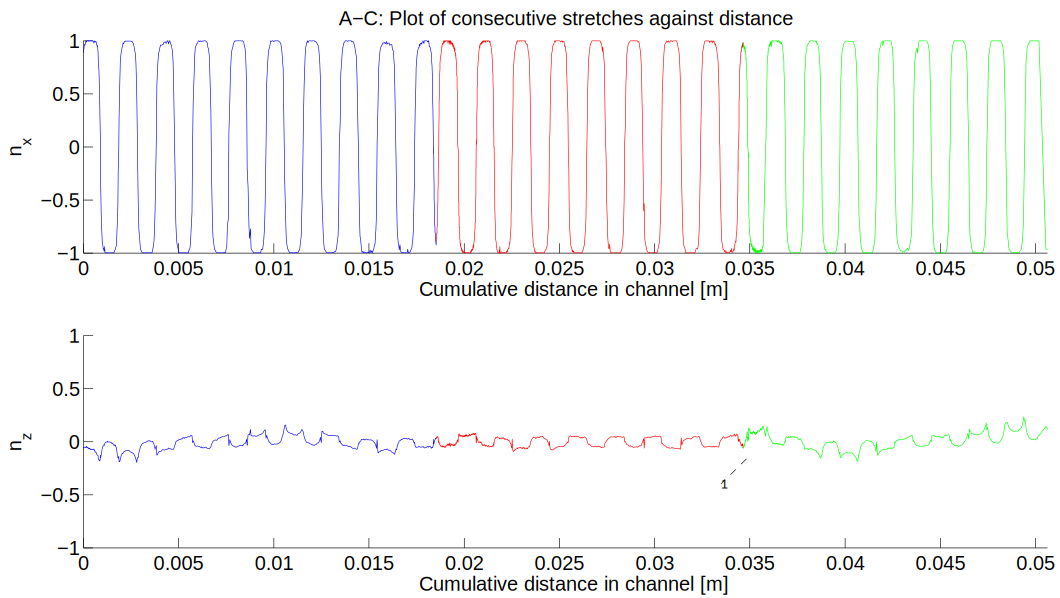
\includegraphics[width=0.7\textwidth]{figures/results/particleA/October_11_Particle_2_run_2_A.pdf}
\end{center}
\caption{Despite being very close to a center orbit there is very little quasi periodic behaviour. The very flattened peaks compared to a low $n_z$ orbit in \ref{fig:orbitparams} are a result of the width compensation discussed in section \ref{sec:width_compensation}.}
\label{fig:particleA1}
\end{figure}

\begin{figure}[H]
\begin{center}
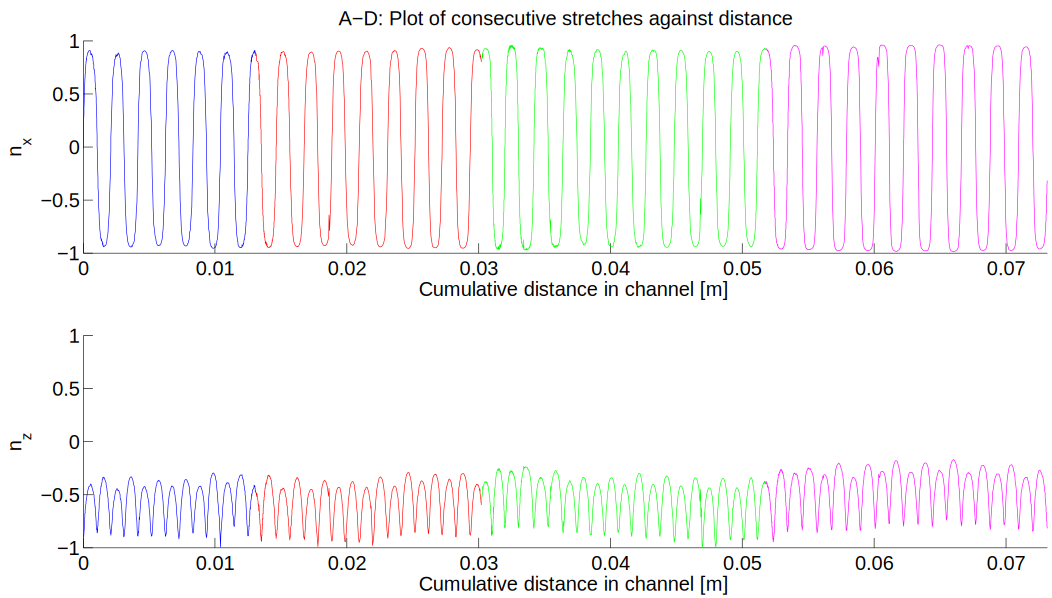
\includegraphics[width=0.7\textwidth]{figures/results/particleA/October_11_Particle_2_run_3_A.pdf}
\end{center}
\caption{A tracked particle with a large $n_z$ component with a very consistent periodic behaviour.}
\label{fig:particleA2}
\end{figure}

\begin{figure}[H]
\begin{center}
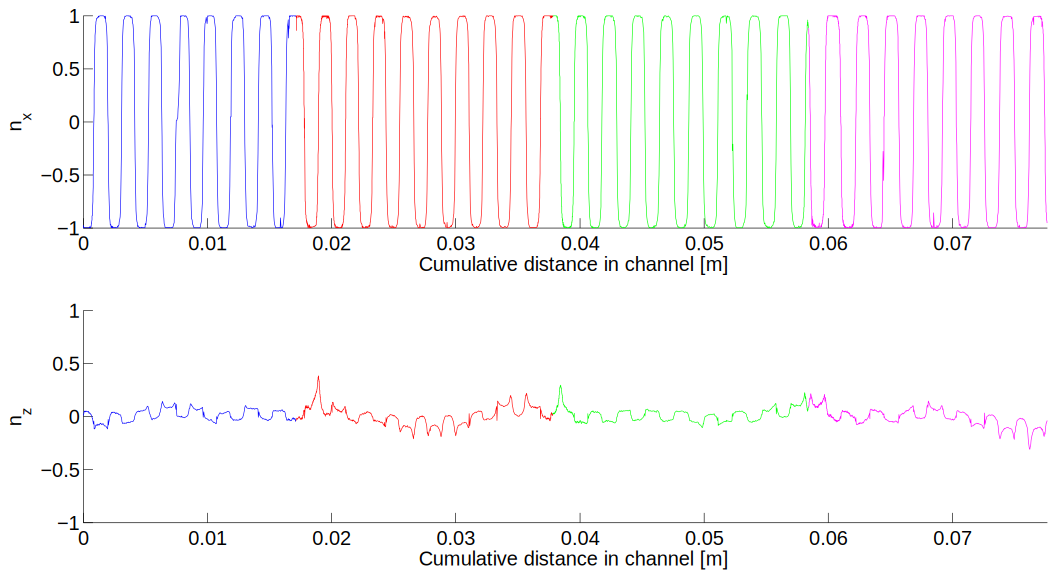
\includegraphics[width=0.7\textwidth]{figures/results/particleA/October_11_Particle_2_run_6_A.pdf}
\end{center}
\caption{The peaks that occur after each reversal are not the cause of a tracking error but can be seen clearly in the films. The cause of such a sudden peak and then reverting back to another orbit is not known and we have no good theoretical explanation for it.}
\label{fig:particleA3}
\end{figure}

\begin{figure}[H]
\begin{center}
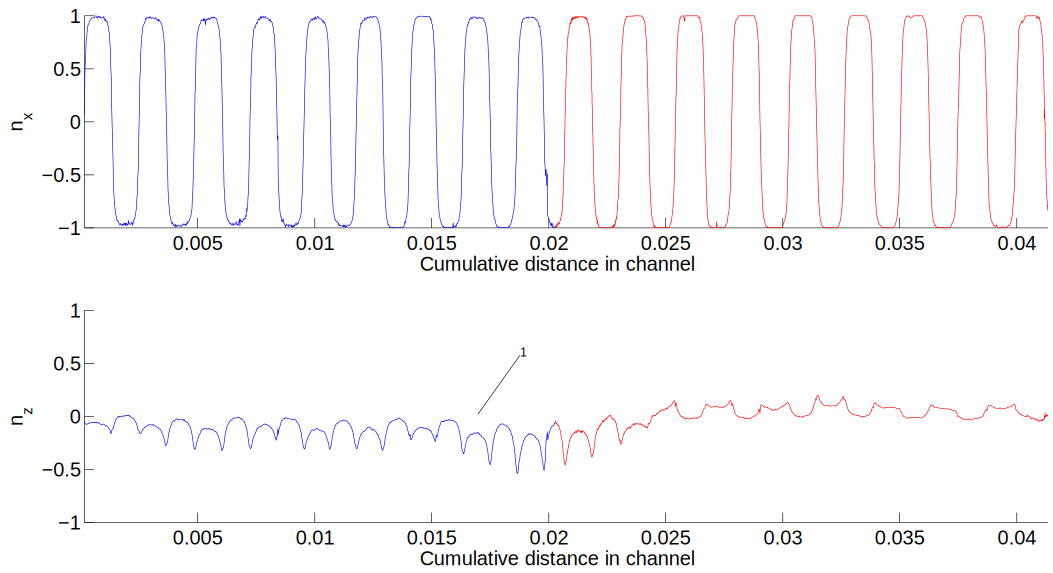
\includegraphics[width=0.7\textwidth]{figures/results/particleA/October_11_Particle_2_run_1_A.pdf}
\end{center}
\caption{The flow is reversed when the particle is at (1) and we see that the orbit appears to change as well.}
\label{fig:particleA4}
\end{figure}

% Put images of matched orbits and selected n_z here.



\section{Particle B}

\subsection{Run 1}
\begin{figure}[H]
\begin{center}
\includegraphics[width=0.7\textwidth]{figures/results/particleB/October_1_Particle_4_run_2_A.pdf}
\end{center}
\caption{The first two stretches match very well as well as the last two. In the reversal between these two there is a large change which begins at (1) where the flow is starting to revert. This reversal also occurs at the end of the channel closer to the pump.}
\label{fig:particleB1}
\end{figure}

\begin{figure}[H]
\begin{center}
\includegraphics[width=0.7\textwidth]{figures/results/particleB/October_1_Particle_4_run_2_D.pdf}
\end{center}
\caption{The speed of the particle against time and against position. In the plot against time there is an extra dip to 0 at around $t=150$ and $t=400$. This occurs only at the end of channel further away from the pump.}
\label{fig:particleB1speed}
\end{figure}

\subsection{Run 2}

\begin{figure}[H]
\begin{center}
\includegraphics[width=0.7\textwidth]{figures/results/particleB/October_1_Particle_4_run_4_A.pdf}
\end{center}
\caption{Mostly constant orbit for large $n_z$. The first and third reversal both change the orbit slightly but the size of the change is exaggerated by $n_z$ being very close to 1. The actual change in orbit can be seen in figure \ref{fig:matchedOrbitsB} to not nearly as these plots suggest. Note also the missing data between the second and third stretch where the particle was lost in tracking for some time, as well as some missing data between the fourth and fifth stretch}
\label{fig:particleB2}
\end{figure}

\begin{figure}[H]
\begin{center}
\includegraphics[width=0.7\textwidth]{figures/results/particleB/October_1_Particle_4_run_5_A.pdf}
\end{center}
\caption{A circular quasi periodic orbit.}
\label{fig:particleB3}
\end{figure}

\begin{figure}[H]
\begin{center}
\includegraphics[width=0.7\textwidth]{figures/results/particleB/October_1_Particle_4_run_3_A.pdf}
\end{center}
\caption{While there is not large change in $n_z$ there seems to be some small variations that could correspond to a bent quasi periodic orbit.}
\label{fig:particleB4}
\end{figure}


